\maketitle
\tableofcontents
\newpage

\section{Zielsetzung}
In diesem Versuch wird die Fourier-Analyse und -Synthese untersucht. Dabei werden
aus Fourier-Komponenten Schwingungen moduliert und bekannte Schwingungen in selbige
zerlegt.

\section{Theorie}
Eine wichtige Rolle beim Fourier-Formalismus spielen periodische Funktionen.
Diese sind definiert durch
\begin{align*}
      f(t + T) &= f(t) \ \text{für zeitliche Periodizität} \\
      f(x + D) &= f(x) \ \text{für räumliche Periodizität} \, .
\end{align*}
Dabei ist $T$ bzw. $D$ die Periodendauer der Funktion; also der Zeitraum,
nachdem $f(t)$ bzw. $f(x)$ wieder den gleichen Wert wie bei $t$ bzw. $x$ hat.
Dafür bieten sich die Sinus- und Cosinus-Funktion an.
Sie finden sich in dem sogennanten Fourierschem Theorem
\begin{equation}
    f(t) = \frac{1}{2} a_0 + \sum_{n = 1}^{\infty} \left(a_n \, \symup{cos} \left(n \frac{2\pi}{T} t \right)
    + b_n \, \symup{sin} \left(n \frac{2\pi}{T} t \right) \right)
    \label{eqn:1}
\end{equation}
wieder, welches erfüllt ist, falls die Reihe aus \eqref{eqn:1} gleichmäßig konvergiert.
Dann gilt für die Koeffizienten $a_n$ und $b_n$
\begin{align}
    a_n &= \frac{2}{T} \int_0^T f(t) \, \symup{cos} \left(n \frac{2\pi}{T} t \right) \symup dt
    \label{eqn:2} \\
    b_n &= \frac{2}{T} \int_0^T f(t) \, \symup{sin} \left(n \frac{2\pi}{T} t \right) \symup dt
    \label{eqn:3}
\end{align}
mit $n \in \mathds{N}$. An \eqref{eqn:2} und \eqref{eqn:3} sieht man, dass in \eqref{eqn:1} nur ganzzahlige
Vielfache der Grundfrequenz $\nu_1 = 1/T$ auftreten. Die Ermittlung der Amplituden
$a_n$ und $b_n$ nennt man Fourier-Analyse. Wenn man \eqref{eqn:2} und \eqref{eqn:3} gegen
die Frequenz aufträgt, erhält man ein Linienspektrum, wie in Abbildung \ref{fig:1} zu sehen.
\begin{figure}
  \centering
  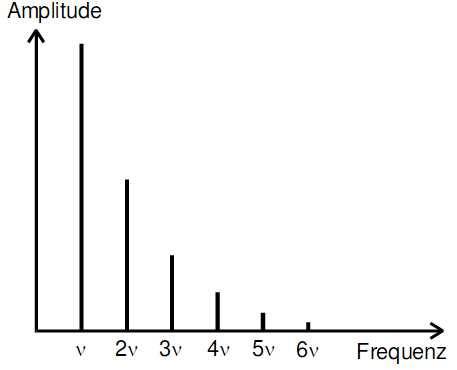
\includegraphics[scale=0.4]{spektrum.png}
  \caption{Linienspektrum einer periodischen Funktion mit Grundfrequenz $\nu$.}
  \label{fig:1}
\end{figure}
Falls $f(t)$ an einer Stelle $t_0$ nicht stetig sein sollte, dann konvergiert \eqref{eqn:1} nicht gleichmäßig
und es tritt eine endliche Abweichung in $f(t_0)$ auf. Diese Abweichung wird für
$n \to \infty$ im Gegensatz zu \eqref{eqn:2} und \eqref{eqn:3} nicht kleiner, sodass sie
in diesem Experiment gut zu beobachten ist, da es sich um Fouriersummen handelt. Die oben
beschriebene Abweichung nennt man Gibbsches Phänomen.

Mit der Fourier-Transformation
\begin{equation}
    g(\nu) = \int_{- \infty}^{\infty} f(t) \, e^{i\nu t} \, \symup dt
    \label{eqn:4}
\end{equation}
lässt sich das ganze Frequenzspektrum $g(\nu)$ einer Funktion $f(t)$ bestimmen,
egal ob sie periodisch ist oder nicht. Falls $f(t)$ periodisch ist, ergibt sich aus
\eqref{eqn:4} eine Reihe aus $\delta$-Distributionen; falls $f(t)$ nicht-periodisch ist,
ist das Frequenzspektrum kontinuierlich. Da es im Experiment nicht möglich ist über
einen unendlichen langen Zeitraum (wie in \eqref{eqn:4} gefordert) zu integrieren,
ergibt sich für jede Funktion $f(t)$ ein kontinuierliches Spektrum. Außerdem werden
Nebenmaxima entstehen, die in der Auswertung gefiltert werden müssen.

\section{Durchführung}

\subsection{Versuchsaufbau}
\subsubsection{Fourier-Synthese}
\begin{figure}
  \centering
  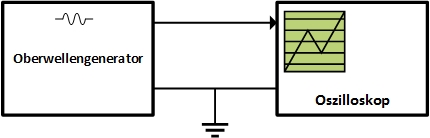
\includegraphics[scale=0.8]{FourierSynthese.jpg}
  \caption{Schaltbild zur Durchführung der Fourier-Synthese \cite{synthese}.}
  \label{fig:2}
\end{figure}
In Abbildung \ref{fig:2} ist der Aufbau zur Durchführung der Fourier-Synthese
zu sehen. Am Oberwellengenerator werden die Fourier-Komponenten überlagert
und die dadurch entstandene Schwingung auf dem Oszilloskop sichtbar gemacht.

\subsubsection{Fourier-Analyse}
\begin{figure}
  \centering
  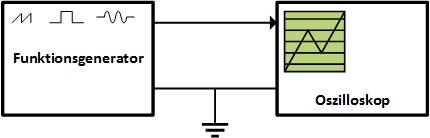
\includegraphics[scale=0.8]{FourierAnalyse.jpg}
  \caption{Schaltbild zur Durchführung der Fourier-Analyse \cite{synthese}.}
  \label{fig:3}
\end{figure}
Um die Fourier-Analyse durchzuführen, wird der Aufbau aus Abbildung \ref{fig:3}
angewandt. Der Funktionsgenerator gibt wahlweise eine der drei Spannungen
(siehe Kapitel \ref{sec:durchfuehrung}) auf das Oszilloskop.

\subsection{Versuchsdurchführung}
\label{sec:durchfuehrung}
\subsubsection{Fourier-Synthese}
Zuerst werden die Oberwellen, für die $n \ge 2$ gilt, mittels Lissajous-Figuren
mit der Sinus-Grundschwingung in Phase gebracht. Dann werden die Fourier-Komponenten
für eine Sägezahn-, eine Dreieck- und eine Rechteckfunktion berechnet (siehe Kapitel \ref{sec:auswertung}).
Dabei sieht man, dass die Amplituden für eine Sägezahn- und eine Rechteckfunktion m
$1/n$ abfällen; während es sich bei der Dreiecksfunktion um einen Proportionalitätsfaktor
$1/n^2$. Mit der Maximalamplitude der Sinus-Schwingung werden alle weiteren Amplituden
der Oberwellen über ein Voltmeter mit den bereits erwähnten Proportionalitätsfaktoren angepasst.
Sodann werden die Oberwellen nacheinander aufsummiert und mittels $\SI{90}{\degree}$ und
$\SI{180}{\degree}$ Phasenverschiebungen entsprechend der gewünschten Funktion angepasst,
bis man alle Oberwellen, die der Generator hergibt, aufsummiert hat. Das Ergebnis lässt
sich auf dem Oszilloskop betrachten.

\subsubsection{Fourier-Analyse}
Am Funktionsgenerator wird eine der drei Funktionen eingestellt. Das Oszilloskop
führt dann die Fourier-Analyse aus, wenn man in den Math-Modus geht. Als nächstes
nimmt man von den Peaks der Hauptmaxima die Amplitude in Abhängigkeit von der
Frequenz auf. Dieser Vorgang wird für die anderen zwei Funktionen wiederholt.

\section{Auswertung}
\label{sec:auswertung}
\subsection{Berechnung der Fourier-Koeffizienten}
\label{sec:koef}
\subsubsection{Rechteckfunktion}
\label{sec:Rechteck}
Die Rechteckfunktion wird wie folgt parametrisiert:
\begin{equation}
R(t)=\left\{\begin{array}{cl} 1, & \mbox{falls }t \in (0, \pi )\\ 0, & \mbox{falls }t \in \{0, \pi, 2\pi \}\\
-1, & \mbox{falls }t \in (\pi, 2\pi ) \; . \end{array}\right.
\end{equation}
Da die Rechteckfunktion ungerade ist, sind alle $a_n = 0$. Es folgt nach \eqref{eqn:3} für die $b_n$:
\begin{equation}
  b_n = \frac{2}{\pi} \int_0^\pi \sin(n t) \symup{d}t = \left\{\begin{array}{cl} 0, & n \mbox{ gerade}\\
  \frac{4}{n \pi}, & n \mbox{ ungerade} \; . \end{array}\right.
\end{equation}
Die Amplituden der Fourierentwicklung fallen also mit $\frac{1}{n}$ ab. Nur ungerade $n$ liefern
Beiträge.
\subsubsection{Dreieckfunktion}
\label{sec:Dreieck}
Die Dreickefunktion wird wie folgt parametrisiert:
\begin{equation}
  D(t) =\frac{2}{\pi}|t| -1 \, , \; t \in [-\pi, \pi).
\end{equation}
Da die Dreieckfunktion gerade ist, sind alle $b_n = 0$. Es folgt nach \eqref{eqn:2} für die $a_n$:
\begin{equation}
  a_n = \left\{\begin{array}{cl} 0, & n \mbox{ gerade}\\
  -\frac{4}{n^2 \pi}, & n \mbox{ ungerade} \; . \end{array}\right.
\end{equation}
Die Amplituden der Fourierentwicklung fallen also mit $\frac{1}{n^2}$. Nur ungerade $n$ liefern
Beiträge.
\subsubsection{Sägezahnfunktion}
\label{sec:Sägezahn}
Die Sägezahnfunktion wird wie folgt parametrisiert:
\begin{equation}
  S(t) =t \, , \; t \in [-\pi, \pi).
\end{equation}
Da die Sägezahnfunktion ungerade ist, sind alle $a_n = 0$. Es folgt nach \eqref{eqn:3} für die $b_n$:
\begin{equation}
b_n = (-1)^{n+1} \frac{2}{n}
\end{equation}
Die Amplituden der Fourierentwicklung fallen also mit $\frac{1}{n}$. Sowohl gerade als auch
ungerade $n$ liefern Beiträge.
\subsection{Fourier-Synthese}
Die Amplitude der Grundfrequenz $A_0$ beträgt \SI{0.614}{\volt}. Zur Erzeugung der jeweiligen
Schwingungsformen werden die Amplituden der n-ten Oberschwingung nach den in Kapitel \ref{sec:koef}
bestimmten Zusammenhängen bestimmt und dementsprechend eingestellt.
\subsubsection{Rechteckschwingung}
Nach dem Entfernen der Phasenverschiebung zwischen den Oberwellen sowie dem Einstellen
der Amplituden nach dem in Kapitel \ref{sec:Rechteck} bestimmten $\frac{1}{n}$ Zusammenhang,
ergibt sich kein Bild auf dem Oszilloskop, das einer Rechteckschwingung nahe kommt.
Durch wahlloses Probieren lässt sich das Ergebnis auf das in Grafik \ref{abb:1} dargestellte
Oszilloskopbild steigern.
\begin{figure}
  \centering
  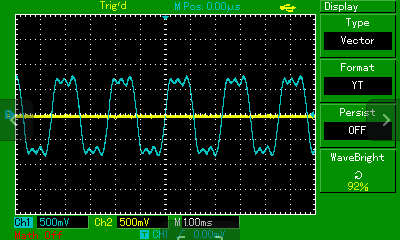
\includegraphics[scale=0.4]{Rechteck.png}
  \caption{Oszilloskopbild der synthetisierten Rechteckschwingung.}
  \label{abb:1}
\end{figure}
\subsubsection{Dreieckschwingung}
Werden die Amplituden wie in Kapitel \ref{sec:Dreieck} eingestellt, ergibt sich das in
Grafik \ref{abb:2} dargestellte Bild auf dem Oszilloskop. Dieses Bild lässt sich durch
Werden die Amplituden  der ungeraden Oberschwingungen wie in Kapitel \ref{sec:Dreieck} mit $\frac{A_0}{n^2}$ eingestellt,
ergibt sich das in Grafik \ref{abb:2} dargestellte Bild auf dem Oszilloskop. Die geraden Oberschwingungen tragen nicht
zur Fourierreihe bei.
\begin{figure}
  \centering
  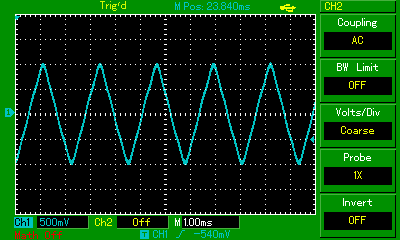
\includegraphics[scale=0.4]{Dreieck.png}
  \caption{Oszilloskopbild der synthetisierten Dreieckschwingung.}
  \label{abb:2}
\end{figure}
\subsubsection{Sägezahnschwingung}
Durch Einstellen nach Kapitel \ref{sec:Sägezahn} ergibt sich das in Grafik \ref{abb:3} dargestellte
Bild.
\begin{figure}
  \centering
  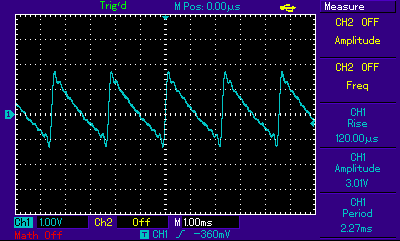
\includegraphics[scale=0.4]{Saegezahn.png}
  \caption{Oszilloskopbild der synthetisierten Sägezahnschwingung.}
  \label{abb:3}
\end{figure}
\section{Fourier-Analyse}
\begin{figure}
  \begin{subtable}{0.6\textwidth}
  \centering
  \begin{tabular}{S S S S S}
    \toprule
    & \multicolumn {2}{c}{Rechteckschw.} & \multicolumn {2}{c}{Dreieckschw.}\\
    $\nu$ / \si{\kilo\hertz} & {$U_{\symup{mes.}}$/\si{\volt}} & {$U_{\symup{erw.}}$/\si{\volt}} &
    {$U_{\symup{mes.}}$/\si{\volt}} & {$U_{\symup{erw.}}$/\si{\volt}} \\
    \midrule
    10 & 8.88 & 8.88 & 5.60 & 5.60 \\
    30 & 2.88 & 2.96 & 0.62 & 0.62 \\
    50 & 1.68 & 1.78 & 0.28 & 0.22 \\
    70 & 1.12 & 1.27 & 0.09 & 0.11 \\
    90 & 0.88 & 0.99 & 0.05 & 0.07 \\
    110 & 0.64 & 0.81 & 0.04 & 0.05 \\
    130 & 0.48 & 0.68 & 0.03 & 0.03 \\
    \bottomrule
    \end{tabular}
    \caption{ }
    \label{sub:1}
    \qquad
  \end{subtable}
  \begin{subtable}{0.3\textwidth}
  \centering
  \begin{tabular}{S S S}
    \toprule
    & \multicolumn {2}{c}{Sägezahnschw.}\\
    $\nu$ / \si{\kilo\hertz} & {$U_{\symup{mes.}}$/\si{\volt}} & {$U_{\symup{erw.}}$/\si{\volt}} \\
    \midrule
    10 & 4.40 & 4.40 \\
    20 & 2.24 & 2.20 \\
    30 & 1.56 & 1.47 \\
    40 & 1.16 & 1.10 \\
    50 & 0.92 & 0.88 \\
    60 & 0.80 & 0.73 \\
    70 & 0.68 & 0.63 \\
    80 & 0.60 & 0.55 \\
    90 & 0.52 & 0.49 \\
    100 & 0.44 & 0.44 \\
    110 & 0.40 & 0.40 \\
    \bottomrule
    \end{tabular}
    \caption{ }
    \label{sub:2}
    \qquad
  \end{subtable}
  \caption{In Tabelle \ref{sub:1} sind die aus der vom Oszilloskop durchgeführten Fourier-Analyse
  der Rechteck- und Dreieckschwingung entnommen Amplituden $U_{\symup{mes.}}$ der jeweiligen Oberschwingungen dargestellt.
  Gleiches findet sich in \ref{sub:2} für die Sägezahnschwingung. Der Funktionsgenerator liefert
  Oberschwingungen von $n \cdot \SI{10}{\kilo\hertz}$. Die Erwartungswerte $U_{\symup{erw.}}$
  wurden nach dem jeweiligen in Kapitel \ref{sec:koef} bestimmten Konvergenzverhalten der Schwingungsformen
  aus der ersten Oberwelle bestimmt.}
\label{abb:4}
\end{figure}
In Abbildung \ref{abb:4} sind die Messwerte der Fourier-Analyse dargestellt. Es zeigt sich,
wie zu erwarten, ein diskretes Spektrum. Weiterhin treten nur bei den Frequenzen Amplituden
auf, die nach den Berechnungen in Kapitel \ref{sec:koef} zu erwarten waren. Im Vergleich mit den
Erwartungswerten zeigen sich Abweichungen, die immer unter \SI{0.2}{\volt} liegen.
Die relativen Abweichungen liegen bei höchstens \SI{29.4}{\percent}. Es zeichnet sich
keine Schwingungsform durch besondere Genauigkeit aus.
\section{Diskussion}
Bei der Synthese zeigen sich starke Abweichungen zwischen den einzelnen Schwingungsformen.
Konnte die Dreieckschwingung sehr gut synthetisiert werden, gibt es bei Rechteck- und Sägezahnschwingung
große Abweichungen von der "Idealform". Dies fällt bei der Rechteckschwingung extrem auf.
Dies ist durch das ausschließliche Beitragen ungerader Oberschwingungen bei einem mit
$1/n$ langsamen Konvergieren der Fourierreihe zu erklären. Die Vermutung liegt nahe,
dass schlicht nicht genug beitragende Oberschwingungen zur Verfügung standen, um die
Schwingungsform vernünftig zu synthetisieren. Auch die sehr gut gelungene Dreieckschwingung
hat nur Beitragende ungerade Oberschwingungen, das Konvergenzverhalten ist mit $1/n^2$
jedoch viel schneller, sodass weniger Summanden benötigt werden um die Schwingungsform
ausreichend genau zu approximieren. Auch die Sägezahnschwingung hat lediglich ein
Konvergenzverhalten wie $1/n$, hier tragen jedoch sowohl gerade als auch ungerade Oberschwingungen
bei. Die Schwingungsform konnte also mit den zur Verfügung stehenden Mitteln besser genähert werden.
Dennoch zeigen sich, insbesondere an den Unstetigkeitsstellen, deutliche Überschwinger, die
sich durch weitere Oberschwingungen sicherlich hätten vermeiden lassen können. Es bietet sich daher
generell die Wiederholung des Versuches mit einem Oberwellengenarator an, der mehr
Oberwellen zur Verfügung stellen kann.\\
\\
Die Abweichungen bei der Fourier-Analyse lassen sich durch die Messmethode erklären.
Die Amplituden der Oberschwingungen wurden mithilfe eines Cursors am Oszilloskop abgelesen.
Wird der Cursor dabei nicht exakt platziert, ergeben sich sofort systematische Fehler.\\
\\
Zusammenfassend zeigt sich eine gute Umsetzbarkeit der Fourier-Analyse. Durch die begrenzten
Leistungsfähigkeit des verwendeten Oberwellengenerators gibt es bei der Fourier-Synthese
jedoch einige Schwierigkeiten. Es können jedoch, abhängig von der Schwingungsform, für
den geringen Aufwand gute Ergebnisse erhalten werden. Lediglich die Rechteckschwingung
bereitet größere Probleme.
\newpage
\nocite{*}
\printbibliography
